\documentclass[eng]{class}
% Publication Title
\title{Movie Reviews: A machine learning project}
% Short title for the header (copy the main title if it is not too long)
\shorttitle{Movie Reviews}
       
% Authors
\author[1]{D. Ligari}
% Author Affiliations
\affil[1]{University of Pavia, Department of Computer Engineering (Data Science), Pavia, Italy}
% Surname of the first author of the manuscript
\firstauthor{Ligari}
%Contact Author Information
\contactauthor{D. Ligari} % Name and surname of the contact author
\email{davide.ligari01@universitadipavia.it} % Contact Author Email
% Publication data (will be defined in the edition)
\publicationdate{\today}
% Place your particular definitions here
\newcommand{\vect}[1]{\mathbf{#1}}  % vectors

\abstract{ 
  This report provides a comprehensive analysis of the steps taken to develop a machine learning model for classifying film reviews. 
  The dataset used in this study is Andrew Maas's \textit{Large Movie Review Dataset}, which includes 50,000 labelled film reviews as either positive or negative.
  Prior to training the model, a preprocessing phase was conducted, which involved creating a vocabulary consisting of all words in the dataset,
  and a bag-of-words (BOW) approach where the number of occurrences of each word in each review was counted. 
  The BOW approach was subsequently used to train the model.\newline
  Different models were then created and compared, 
  incorporating various preprocessing techniques, including stemming and the removal of common and meaningless words from the vocabulary.\newline 
  The report also includes the use of different classifiers, such as logistic regression and multinomial Naive Bayes. 
  }
\keywords{ Machine Learning • Classification • Sentiment Analysis • Logistic Regression • Multinomial Naive Bayes}
\date{\today}
% Start document
\begin{document}
% Include title, authors, abstract, etc.
\maketitle
\thispagestyle{fancy}
%Figures and tables must be cited in the text and explained in detail. Do not forget to add a caption to each figure/table/
\section{Introduction}
\firstword{I}{n}
recent years, the exponential growth of digital media and the internet has led to an unprecedented amount of content being produced and consumed on a daily basis.
One of the most popular forms of digital media is film, with millions of reviews available online from a variety of sources. With this vast amount of data available,
it has become increasingly challenging to manually process and classify this information.
By using large datasets and advanced algorithms, machine learning models can accurately classify reviews based on their content.
In this report, is presented a thorough analysis of the steps taken to create a machine learning model for classifying film reviews.
\section{Dataset}
The dataset used in this study is Andrew Maas's \textit{Large Movie Review Dataset},
which includes 50,000 labelled film reviews equally distributed in the two classes - positive and negative.
The dataset is already divided into a training set of 25,000 reviews, a validation set of 12,500, and a test set of 12,500,
which allows for the evaluation of the model's performance on unseen data.
\section{Model creation}
The initial step in building the model is to construct the vocabulary, which is a comprehensive list of all words present in the dataset.
The vocabulary was generated by processing all training reviews, removing any punctuation, and adding each unique word to the vocabulary only once.\newline
Afterward, the vocabulary was sorted alphabetically and filtered to retain only a subset of the most relevant words.
The size of the vocabulary is a crucial parameter that can be adjusted to enhance the model's performance.\newline
Once the vocabulary has been created, the next step is to extract meaningful features from the dataset.
In this study, a bag-of-words (BOW) approach has been used, which counts the number of occurrences of each word in each review.
Thorough the bag of words, the reviews are represented in a structured and quantitative way, making it possible to train machine learning models to accurately classify them.\newline
Now the data are ready to be used to train the model. In this study,the multinomial Naive Bayes classifier has been used.
Given a BoW feature vector x the multinomial NB model predicts the class $\hat{y}$ as follows:
\begin{equation}
  \hat{y} = \mathop{argmax}_{y \in \{0,1\}} \sum_{j=0}^{n-1} x_j \log\pi_{y,j}+\log P(y)
\end{equation}
where $\pi_{y,j}$ represents the probability that a randomly selected word from a document belonging to class y is the j-th word in the vocabulary.
The term P(y) refers to the prior probability for class y.
\subsection{Variants}
In this study, we analyzed different variants of our model by training it with various vocabularies.
In the first variant, we removed the most common, meaningless words such as articles, prepositions, and conjunctions, among others.
In the second one, the stemming technique has been applied, to reduce words to their root form, in order to reduce the vocabulary size, and so, improve the performance of the model.
In the third variant, both techniques has been combined, to create a more comprehensive vocabulary.
\section{Model evaluation}
\subsection{Effect of the vocabulary size}
The vocabulary size is a crucial parameter that affects the performance of the model.
A vocabulary that is too small may not contain enough information to accurately classify reviews,
while a vocabulary that is too large may include irrelevant words that negatively impact the model's performance.
When the vocabulary size is too large, the model may assign a high weight to meaningless words, which can reduce its ability to identify the most relevant ones.\newline
However, as shown in Figure \ref{fig-1}, increasing the vocabulary size can improve the test accuracy of the model, up to a certain point.
In this study, the maximum test accuracy of approximately 0.83 was achieved for a vocabulary size of 2000 words.

\subsection{Variants comparison}
The results presented in Figure \ref{fig-1} demonstrate that the model without the most common words achieves a higher accuracy compared to the other two models.
Specifically, the model using the whole vocabulary shows a lower accuracy than the model without the most common words.
Additionally, the model with stemming has a lower accuracy than the model without the most common words, but performs better than the model using both techniques. \newline
These findings suggest that removing the most common words from the vocabulary has a positive impact on the accuracy of the model,
while stemming can have a slightly negative effect.
One possible explanation for these results is that the most common words in the dataset may not carry much semantic meaning and can introduce noise into the model.
On the other hand, stemming can potentially remove important distinctions between words and reduce the model's ability to differentiate between them.
\begin{figure}[h]
  \centering
  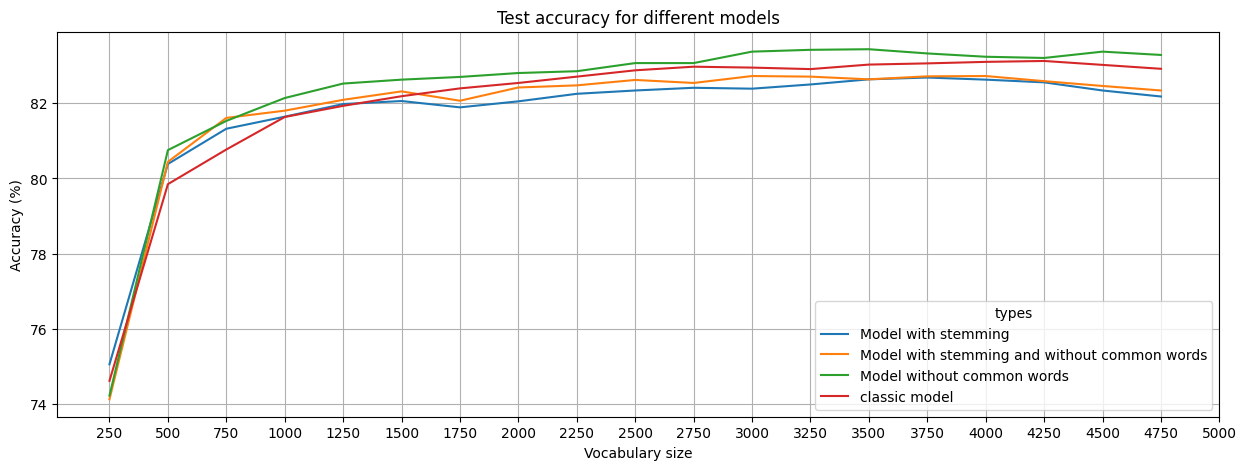
\includegraphics[width=.8\columnwidth]{images/modelComp.png}
  \caption{Comparison of the models for different vocabulary sizes}
  \label{fig-1}
\end{figure}
\subsection{Most impactful words}
Figure \ref{fig-2} displays the most impactful words for the model using a 2000-size vocabulary without the most common words.
The results show that the model performs well, giving significant importance to adjectives that convey a clear positive or negative sentiment.
This outcome can be attributed to the effectiveness of the vocabulary size which enable the model to focus on the most relevant words for classification.
However, when the vocabulary size increases to 5000, the model's performance degrades, as seen in Figure \ref{fig-3}.
The model appears to give importance to words that do not necessarily carry a clear sentiment, leading to a less effective classification.


\begin{figure}[h]
  \begin{subfigure}{.5\linewidth}
    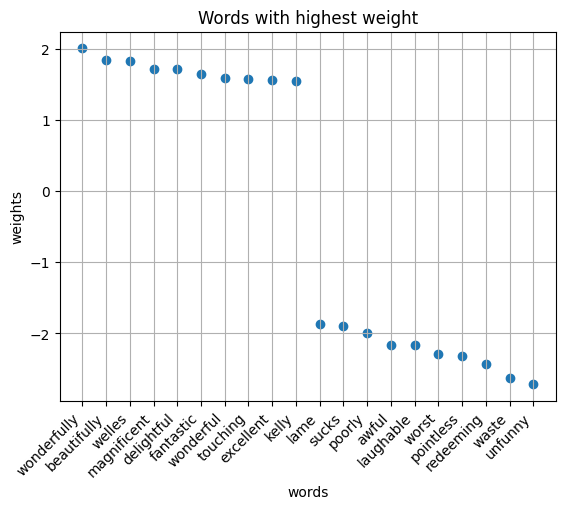
\includegraphics[width=.8\columnwidth]{images/words.png}
  \end{subfigure}%
  \begin{subfigure}{.5\linewidth}
    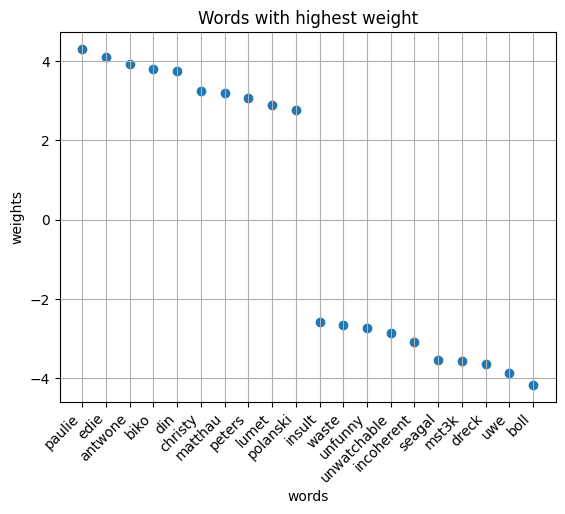
\includegraphics[width=.8\columnwidth]{images/words5000.png}
  \end{subfigure}
  \caption{Most impactful words, for the model without common words,on the left is used vocabulary size =2000, on the right the vocabulary size is equal to 5000}
  \label{fig-2}
\end{figure}

\subsection{Worst errors on the test set}
In Figure \ref{fig-3}, are presented the 20 reviews that were misclassified with high confidence.
These reviews were predicted to belong to a class that was different from their actual class.
\begin{figure}[h]
  \centering
  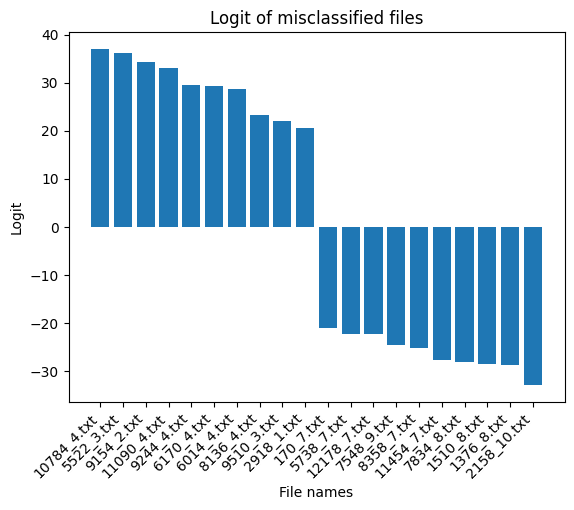
\includegraphics[width=.5\columnwidth]{images/missclassified.png}
  \caption{Logit for misclassified reviews}
  \label{fig-3}
\end{figure}

\section{Logistic regression}
Also a logistic regression model has been trained and compared to the Naive Bayes classifier. To reduce training time, it is employed mini-batch gradient descent instead of batch gradient descent.
Our results indicate that the logistic regression model slightly outperformed the Naive Bayes model, achieving a train accuracy of approximately 88.976\% and a test accuracy of 85.928\%.
Figure \ref{fig-4} shows the most significant words, which are similar to those identified by the Naive Bayes classifier, but with different weights assigned to them.
\begin{figure}[h]
  \centering
  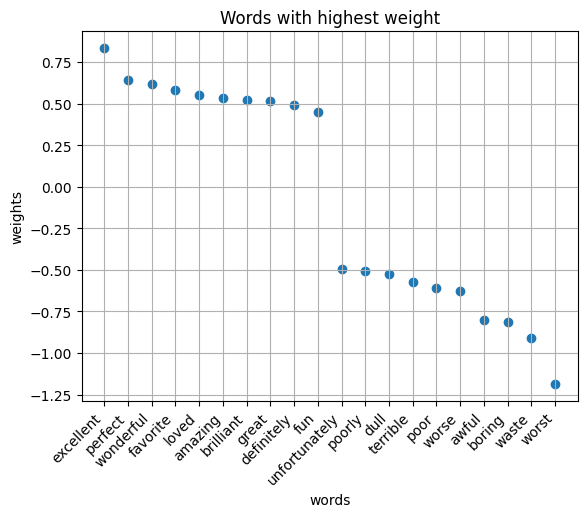
\includegraphics[width=.5\columnwidth]{images/lrwords.png}
  \caption{Most meaningful words for logistic regression}
  \label{fig-4}
\end{figure}

\section{Declaration}
I affirm that this report is the result of my own work and that I did not share any part of it with anyone
else except the teacher.
%\section{References}
%Insert bibliographical references (if any) you might have used for your lab activities.
\end{document}